\documentclass{beamer}
\usetheme[compress]{Singapore}
\setbeamerfont{footnote}{size=\tiny}


\usepackage{amsmath}
\usepackage{mathrsfs}
\usepackage{amssymb}
\usepackage{feynmp}
\usepackage{bm}
\usepackage{mathtools}

\newcommand{\bpar}[1]{\left( #1 \right)}                  % big parentheses
\newcommand{\bra}[1]{\left \langle #1 \right \vert}
\newcommand{\ket}[1]{\left \vert #1 \right \rangle}
\newcommand{\comm}[2]{\left[ #1 , #2\right]}
\newcommand{\qop}[1]{\mathscr{#1}}
\newcommand{\mat}[1]{\boldsymbol{#1}}
\newcommand{\dbar}[2]{\left\langle \left. #1 \right\vert \left\vert #2 \right.\right\rangle}
\renewcommand{\exp}[1]{\mathrm{exp}\bpar{#1}}


\newcommand\blfootnote[1]{%
  \begingroup
  \renewcommand\thefootnote{}\footnote{#1}%
  \addtocounter{footnote}{-1}%
  \endgroup
}
\renewcommand*\footnoterule{}

\title[]{Studying Semi--Classical Molecular Light--Matter Interaction through
Time--Dependent Density Functional Theory (TD-DFT)}
\author[Li Research Group, University of Washington]{
\\[1\baselineskip]
David Williams--Young \\
Department of Chemistry \\
University of Washington \\
Li Research Group
}

\date{\today}

\begin{document}

% Title Page
\begin{frame}
\titlepage
\end{frame}


%%%%% OUTLINE SECTION
\section{Outline}


% Outline
\begin{frame}
\frametitle{Outline}

\begin{itemize}
  \item Semi--Classical Molecular Light--Matter Interaction 
  \item Density Functional Theory (DFT)
  \item Real--Time Time--Dependent Density Functional Theory (RT-TD-DFT)
  \item Some Fun Results
  \item Chebyshev Expansion of the Quantum Propagator
\end{itemize}
\end{frame}

%%%%% THEORY SECTION
\section{Theory}

% Molecular Scattering (1)
\begin{frame}
\frametitle{Semi--Classical Molecular Light--Matter Interaction}
\begin{columns}
\begin{column}{0.5\textwidth}
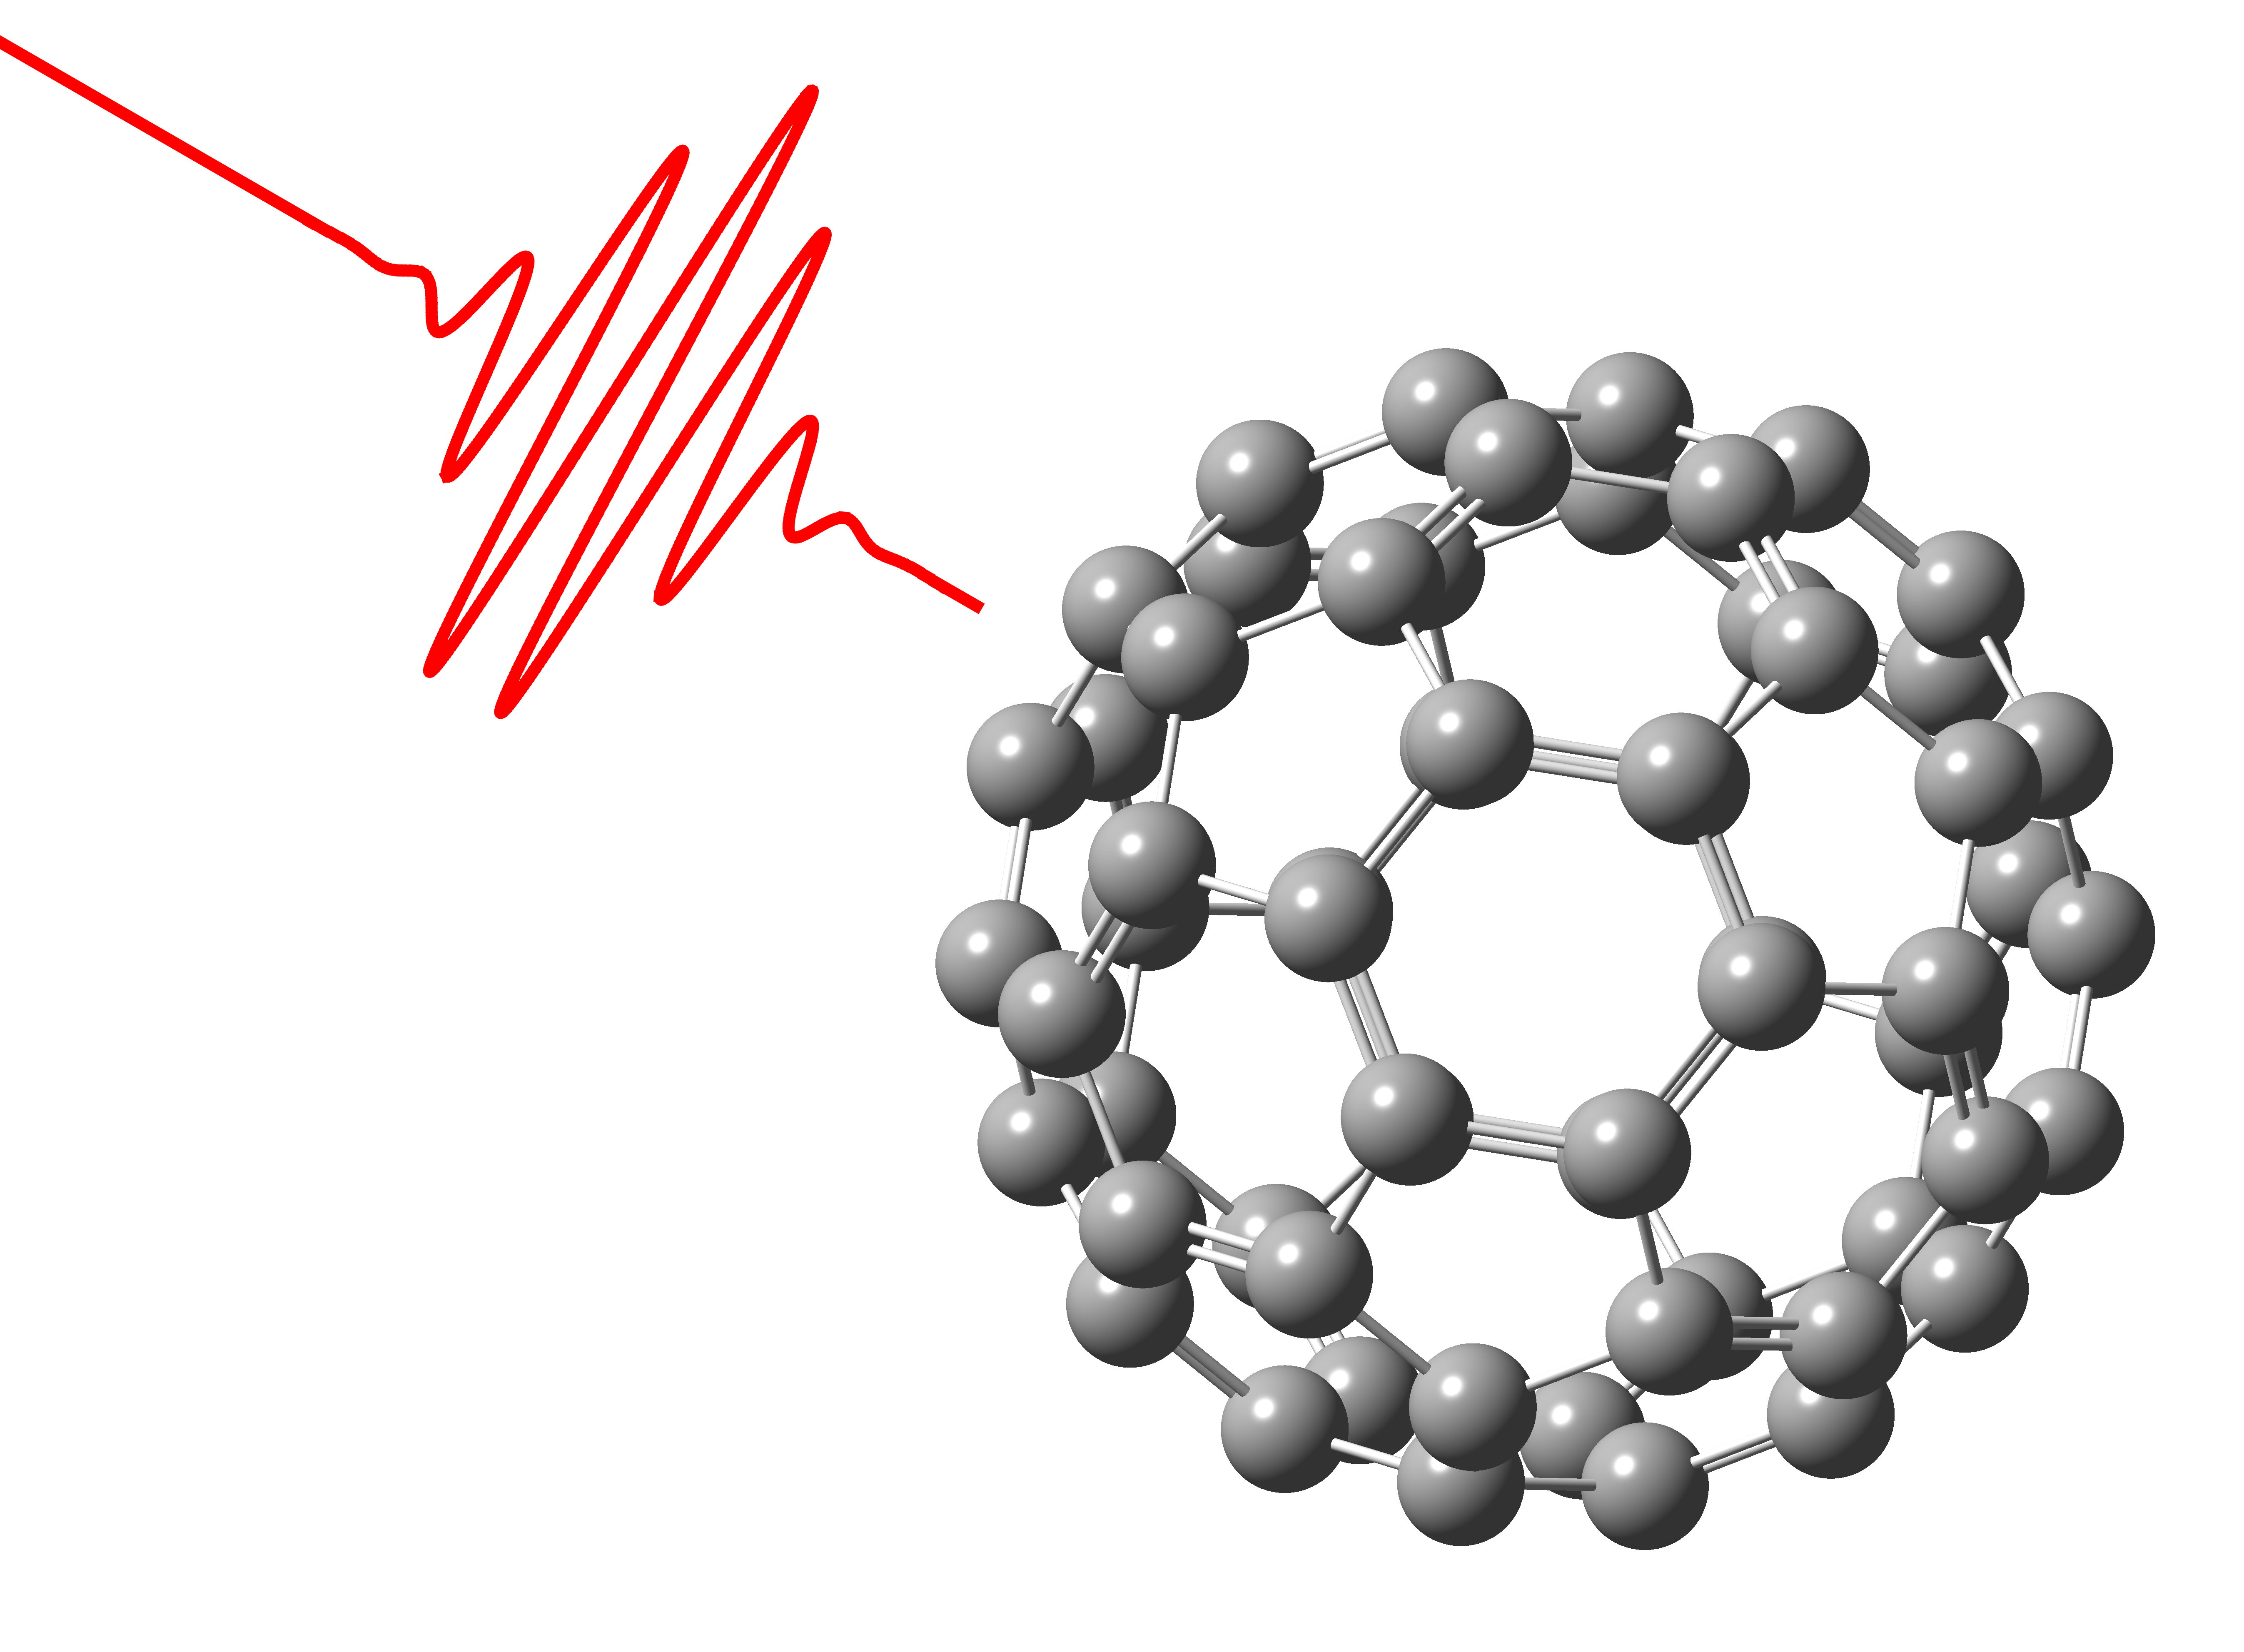
\includegraphics[width=\textwidth]{BMF_pulse}
\end{column}
\begin{column}{0.5\textwidth}
\begin{itemize}
  \item Simple Absorption
  \item Circular Dichroism (CD)
  \item High Harmonic Generation (HHG)
  \item Vibrational Spectroscopy
  \begin{itemize}
    \item Infrared (IR)
    \item Raman
  \end{itemize}
\end{itemize}
\end{column}
\end{columns}
\end{frame}


\begin{frame}
\frametitle{Semi--Classical Molecular Light--Matter Interaction}

(For our purposes) quantum mechanics is governed by the Schr\"{o}dinger (or Dirac--Coulomb--Breit)
equations
\begin{equation*}
\mathcal{H}(t)\ket{\Psi} = \mathrm{i}\partial_t\ket{\Psi} \qquad \mathcal{H}(t) = \mathcal{H}_0 + \mathcal{V}(t)
\end{equation*}

The the presence of an electric field, $\mathbf{E}(t)$
\begin{equation*}
\mathcal{V}(t) = -A_i(t) p^i \qquad \mathbf{A}(t) = \int_{0}^t \mathbf{E}(t') \mathrm{d}t'
\end{equation*}

It is often advantageous to work in the so called length gauge, such that
\begin{equation*}
\mathcal{V}(t) \mapsto \mathcal{V}'(t) = - E_i(t) r^i
\end{equation*}

\end{frame}

\begin{frame}
\frametitle{Semi--Classical Molecular Light--Matter Interaction}

Using time--dependent perturbation theory, we find the absorption probability at a given
frequency may be written in terms of the dipole--dipole polarizability tensor, $\boldsymbol{\alpha}$
\begin{equation*}
S(\omega) \propto \omega \mathrm{Im}\left(\mathrm{Tr}[\boldsymbol{\alpha}(\omega)]\right)
\end{equation*}
~\\
~\\
Within the dipole--approximation, $\boldsymbol{\alpha}$ is related to the 
time--dependent electric dipole, $\boldsymbol{\mu}(t)$ by
\begin{equation*}
\mu_i(t) = \int_0^t \alpha_{ij}(t' -t) E_j(t') \mathrm{d}t' \implies \mu_i(\omega) = \alpha_{ij}(\omega) E_j(\omega)
\end{equation*}

\end{frame}

\begin{frame}
\frametitle{Semi--Classical Molecular Light--Matter Interaction}

\begin{columns}
\begin{column}{0.45\textwidth}
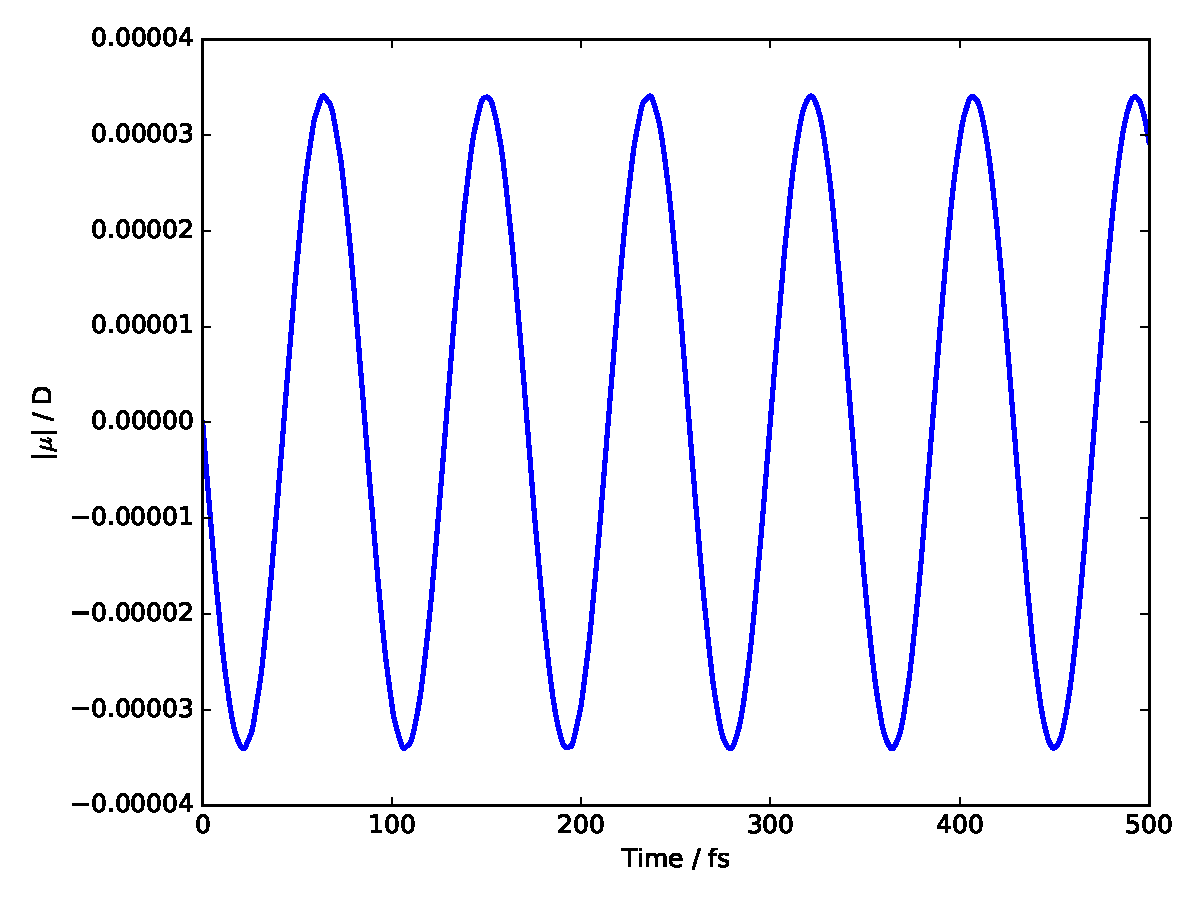
\includegraphics[width=\textwidth]{na_fss_dipole}
\end{column}
\begin{column}{0.1\textwidth}
$\xRightarrow[(Pade)]{\text{FFT}}$
\end{column}
\begin{column}{0.45\textwidth}
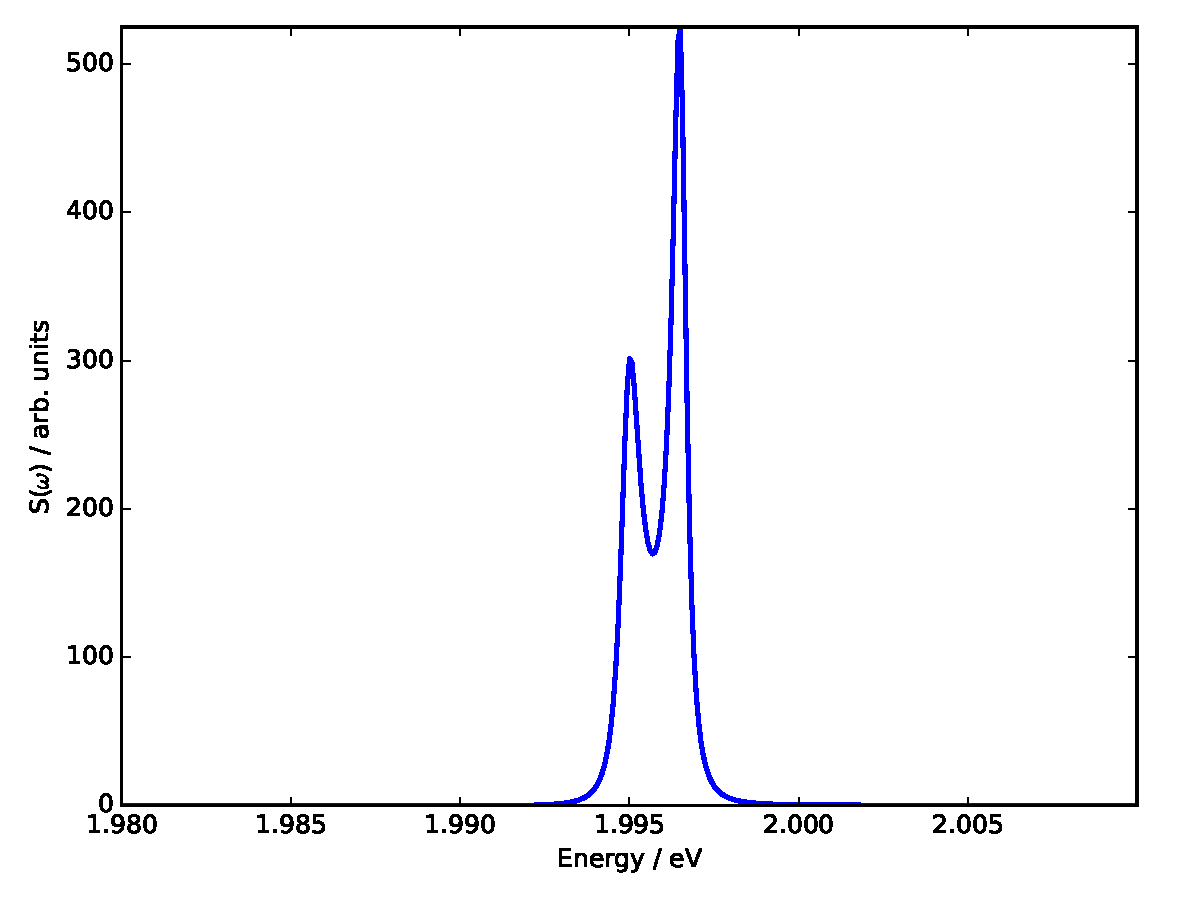
\includegraphics[width=\textwidth]{na_fss}
\end{column}
\end{columns}
\end{frame}

\begin{frame}
\frametitle{Semi--Classical Molecular Light--Matter Interaction}
\begin{center} 
\LARGE How to obtain $\boldsymbol{\mu}(t)$ given $\mathbf{E}(t)$?
\end{center}
~\\
~\\
\begin{center}
\LARGE \bf
Solve the TDSE (TD--DCBE) Obviously! 
\end{center}
\end{frame}

%%%%% DFT SECTION
\section{DFT}

% Hohenberg-Kohn DFT
\begin{frame}
\frametitle{Density Functional Theory (DFT)}
\blfootnote{Hohenberg, P.; Kohn, W.; \emph{Phys. Rev.} \textbf{1964}, \emph{136}, B864}

The Hohenberg--Kohn theorems guarantee the following:
\begin{enumerate}
  \item The total energy of a fermionic system is a unique functional of the density, $F[\rho(\mathbf{r})]$.
  \item $F[\rho(\mathbf{r})]$ obtains its minimum value iff it is evaluated at the ground state density $\rho_G$.
\end{enumerate}

\begin{itemize}
  \color{green}
  \item Formally exact given $F$
  \item Trivially extends to relativistic treatments.
  \item No orbitals!
\end{itemize}

\begin{itemize}
  \color{red}
  \item $F$ is not known for non--trivial systems (jellium)
  \item Kinetic energy contributions in this form is exceptionally difficult.
\end{itemize}

\end{frame}

% Kohn-Sham DFT
\begin{frame}
\frametitle{Kohn--Sham Density Functional Theory (KS--DFT)}
\blfootnote{Kohn W.; Sham, L. J.; \emph{Phys. Rev.} \textbf{1965}, \emph{140}, A1133}

Kohn and Sham introduced a method to obtain the kinetic energy contribution
within a mean field, Slater determinant picture
\begin{equation*}
\mathcal{H}^{KS} = \frac{1}{2}\Delta + \mathcal{V}(\mathbf{r}) + 
  \int \mathrm{d}^3\mathbf{r}'\text{ } \frac{\rho(\mathbf{r}')}{\vert \mathbf{r-r}' \vert} +
  \frac{\delta E^{xc}[\rho(\mathbf{r})]}{\delta \rho(\mathbf{r})}
\end{equation*}

\begin{equation*}
\mathcal{H}^{KS} \phi_i(\mathbf{r}) = \epsilon_i\phi_i(\mathbf{r})
\end{equation*}


\begin{itemize}
  \color{green}
  \item Again, formally exact given the exact $E^{xc}$
  \item Able to easily evaluate kinetic energy
  \item Still trivially extendable to relativistic theory
\end{itemize}

\begin{itemize}
  \color{red}
  \item $E^{xc}$ is still not known (we have to guess)
  \item Orbitals introduce complications over density--only methods
\end{itemize}
\end{frame}

% KSDFT Finite Basis
\begin{frame}
\frametitle{KS--DFT within a Finite Basis}
\blfootnote{Pople, J. A.; Gill, P. M. W.; Johnson, B. G. \emph{Chem. Phys. Lett.} \textbf{1992}, \emph{199(6)}, 557.}

Casting into the mean--field picture allows for a simple expansion
of the KS--DFT equations in a finite basis $\{\chi(\mathbf{r})\}$
\begin{equation*}
F_{\mu\nu}^{KS} C_{\nu p} = S_{\mu\nu}C_{\nu p} \epsilon_p \qquad \quad
F_{\mu\nu}^{KS} = h_{\mu\nu} + J_{\mu\nu} + V^{xc}_{\mu\nu}
\end{equation*}

\begin{equation*}
X_{\mu\nu} = \int \mathrm{d}^3\mathbf{r}\text{ } \chi_\mu(\mathbf{r}) \mathcal{X} \chi_\nu(\mathbf{r})
\qquad \quad V^{xc}_{\mu\nu} = \int \mathrm{d}^3\mathbf{r}\text{ } 
  \frac{\delta E^{xc}[\rho(\mathbf{r})]}{\delta \rho(\mathbf{r})}
  \chi_\mu(\mathbf{r}) \chi_\nu(\mathbf{r})
\end{equation*}

Each molecular orbital is then expanded in the basis
\begin{equation*}
\phi_p(\mathbf{r}) = C_{\mu p} \chi_\mu(\mathbf{r}) \qquad C_{\mu p} \in \mathbb{C}
\end{equation*}
\end{frame}

% RelKSDFT
\begin{frame}
\frametitle{Relativistic Extensions of DFT}

\begin{itemize}
  \item The HK theorems have been shown to be Lorentz covariant with the replacement
  of the density $\rho$, with the 4--current $j^\mu$.

  \item Given the exact functional, we may develop an analogous relativistic Kohn--Sham
  equation (Dirac--Kohn--Sham),
  \begin{equation*}
    \mathcal{H}^{DKS} = c\alpha_\mu p^\mu + c^2\beta + \alpha_\mu \mathcal{V}_s^\mu(\mathbf{r})
  \end{equation*}

  \item We may cast into a finite basis
  \begin{equation*}
    F_{\mu\nu}^{DKS} C_{\nu p} = S_{\mu\nu}C_{\nu p} \epsilon_p \qquad C_{\nu p} \in \mathbb{C}^4
  \end{equation*}
\end{itemize}
\end{frame}

% 2C
\begin{frame}
\frametitle{Relativistic Extensions of DFT}
%\frametitle{Approximate Two--Component KS Methods}

\begin{center} \bf \LARGE Four component KS methods are hard! \end{center}
\begin{itemize}
  \item Not variationally bound from below (Positrons!)
  \item No logical separation of physical observables
  \item Includes information not generally useful for Chemistry
  \item Large computational memory bottleneck
\end{itemize}

\end{frame}

% 2C
\begin{frame}
\frametitle{Approximate Two--Component KS Methods}

Formally, there exists a unitary operator, $\mathcal{U}$, that folds the information
contained in the positronic part of the wave function into the electronic part.
\begin{equation*}
\mathcal{U} : \ket{\Psi^\mathrm{4C}} \rightarrow \ket{\Psi^\mathrm{2C}} \in \mathbb{C}^2
\end{equation*}

\begin{itemize}
  \color{green}
  \item Variationally bound from below
  \item Separates physical observables (SO coupling, etc)
  \item Contains information from the positronic component without treating it explicitly
\end{itemize}

\begin{itemize}
  \color{red}
  \item In general, an exact $\mathcal{U}$ is not known for the many--body wave function.
  (Must use approximate decoupling schemes)
\end{itemize}

\end{frame}


% 2C
\begin{frame}
\frametitle{Approximate Two--Component KS Methods}

Using the X2C method for $\mathcal{U}$, the DKS equations become
\begin{equation*}
F^{X2C}_{\mu\nu} C_{\nu p} = S_{\mu\nu} C_{\nu p} \epsilon_p \qquad C_{\nu p} \in \mathbb{C}^2 \text{ (or }\mathbb{H})
\end{equation*}
~\\
~\\
Aside: 

This allows for a convenient decomposition
\begin{equation*}
F_{\mu\nu}^{X2C} = F_{\mu\nu}^S \otimes I_2 + F_{\mu\nu}^k \otimes \sigma_k
\end{equation*}


\begin{equation*}
XY = \bpar{X^SY^S + X^kY_k} \otimes I_2 + \bpar{X^S Y^k + X^k Y^S + \mathrm{i}\varepsilon_{kij}X^iY^j}\otimes \sigma_k
\end{equation*}
\begin{center} (This will become very useful) \end{center}
\end{frame}

% Properties
\begin{frame}
\frametitle{Properties through KS--DFT}

Given a static operator $\mathcal{O}$ and basis representation $O_{\mu\nu}$, the (time--dependent) expectation value
of this operator is given as
\begin{equation*}
\langle \mathcal{O}(t) \rangle = \mathrm{Tr}[\mathbf{P}(t)\cdot\mathbf{O}]
\end{equation*}

In particular for 2C methods, if $\mathcal{O}$ doesn't depend on spin, this reduces to
\begin{equation*}
\langle \mathcal{O}(t) \rangle = \mathrm{Tr}[\mathbf{P}^S(t)\cdot\mathbf{O}]
\end{equation*}

\end{frame}

%%%%% TDDFT SECTION
\section{TD-DFT}

\begin{frame}
\frametitle{Real--Time Time--Dependent Density Functional Theory (RT-TD-DFT)}
\blfootnote{Li, X.; Smith, S. M.; Markevitch, A. N.; Romanov, D. A.; Levis, R.
J.; Schlegel, H. B. \emph{PCCP} \textbf{2005}, 7, 233−239.}

The dynamics of the KS electronic density is given by the Liouville--von Neumann (LvN) equation
\begin{equation*}
  \mathrm{i}\partial_t\mathbf{P}(t) = \comm{\mathbf{F}(t)}{\mathbf{P}(t)} \qquad F_{\mu\nu}(t) = h_{\mu\nu} + G_{\mu\nu}[\mathbf{P}(t)] + V_{\mu\nu}(t)
\end{equation*}
~\\

In practice, we integrate the LvN via the modified midpoint unitary transformation (MMUT)
method
\begin{equation*}
\mathbf{P}(t_{k+1}) = \mathbf{U}(t_k)^\dagger \mathbf{P}(t_{k-1}) \mathbf{U}(t_k)
\end{equation*}
\begin{equation*}
\mathbf{U}(t_k) = \exp{-2\mathrm{i}(\Delta t) \mathbf{F}(t_k)}
\end{equation*}

\end{frame}

%%%%% RESULTS SECTION
\section{Results}

\begin{frame}
\frametitle{Na D--Line Splitting}

\begin{minipage}[h!]{0.45\textwidth}
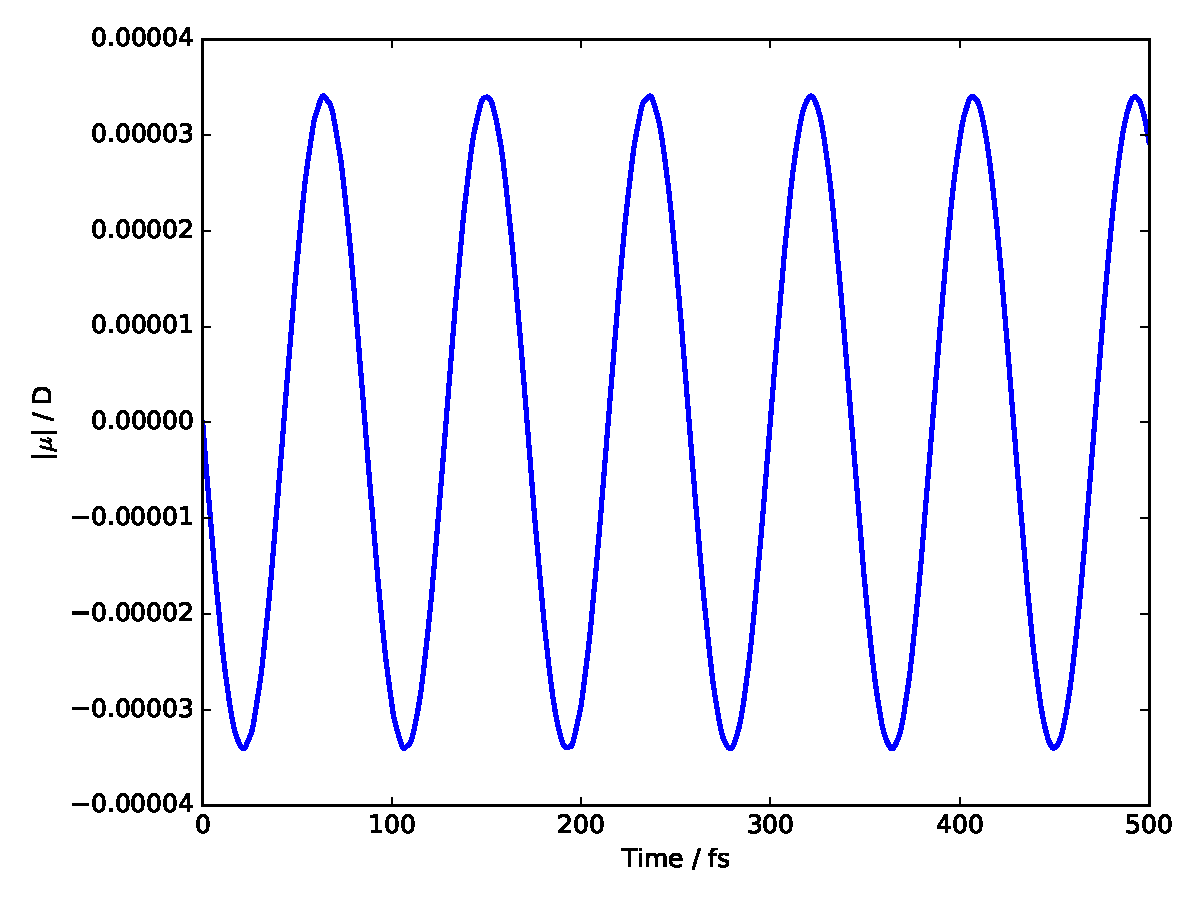
\includegraphics[width=\textwidth]{na_fss_dipole}\\
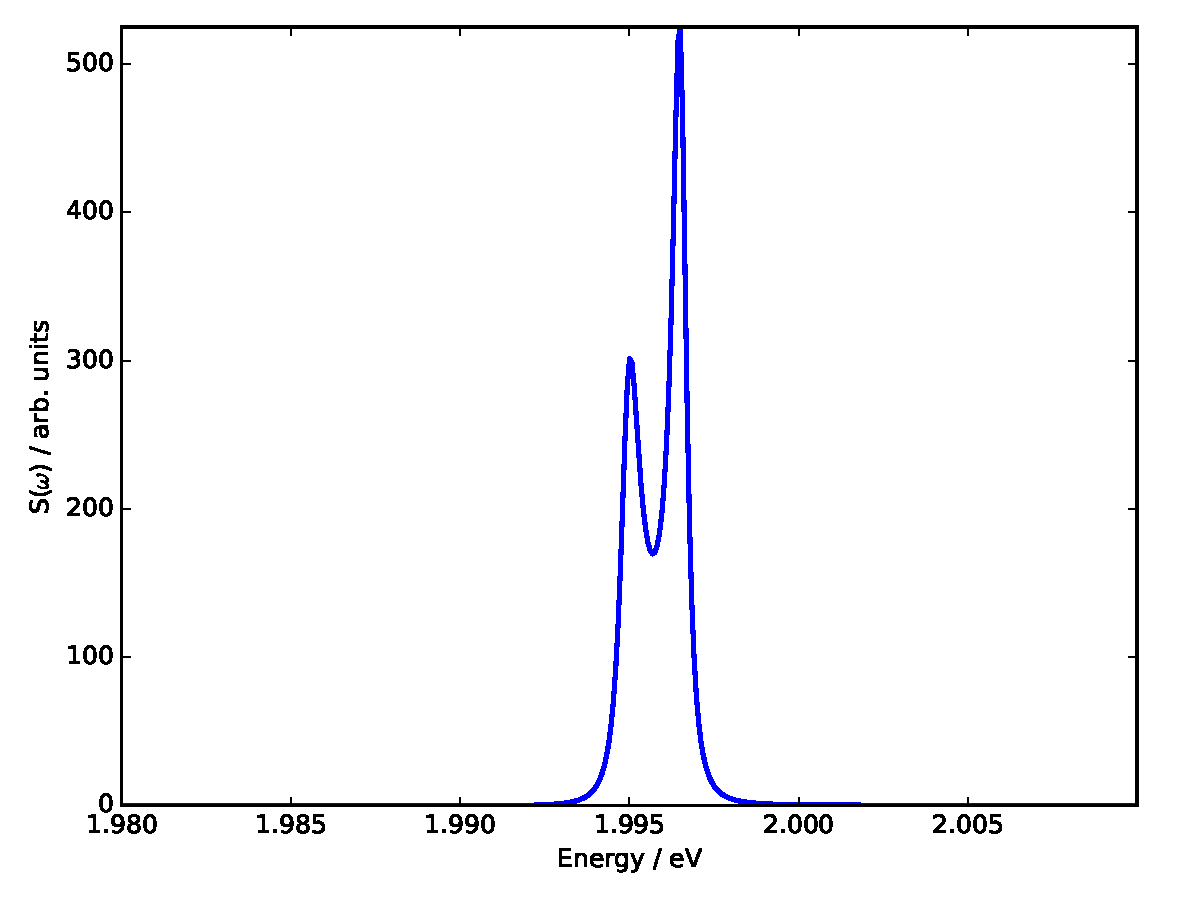
\includegraphics[width=\textwidth]{na_fss}
\end{minipage}
\blfootnote{http://www.astrosurf.com/buil/spectro\_apn/result.htm}
\blfootnote{http://hyperphysics.phy-astr.gsu.edu/hbase/quantum/sodzee.html}
\begin{minipage}[h!]{0.50\textwidth}

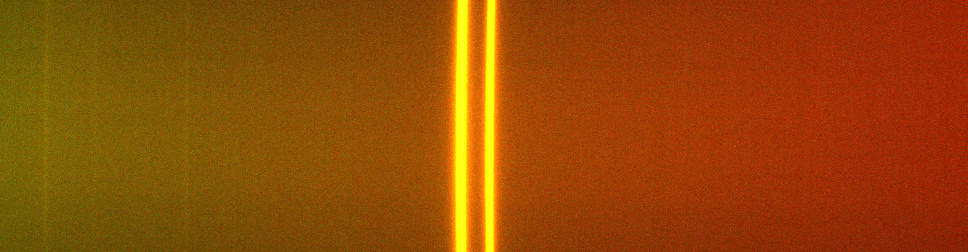
\includegraphics[width=\textwidth]{NaLines}
%http://www.astrosurf.com/buil/spectro_apn/result.htm

\begin{minipage}[h!]{0.5\textwidth}
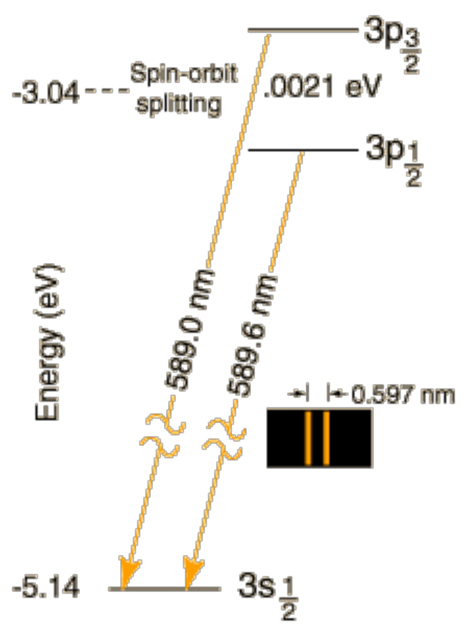
\includegraphics[width=\textwidth]{Nadoub}
%http://hyperphysics.phy-astr.gsu.edu/hbase/quantum/sodzee.html
\end{minipage}
\begin{minipage}[h!]{0.47\textwidth}

\small
~\\
\textbf{Na X2C/6-31G}
\vspace{-0.5cm}
\begin{table}
\begin{tabular}{|l|l|}
\hline
E (eV) & $S(\omega)$ \\
\hline
\hline
1.9950 & 301.2\\
1.9965 & 524.8\\
\hline
\end{tabular}
\end{table}
\vspace{-0.5cm}
\begin{table}
\begin{tabular}{|l|l|}
\hline
 & FSS (meV) \\
\hline
\hline
Theor & 1.5\\
Exp & 2.1\\
\hline
\end{tabular}
\end{table}
\end{minipage}

\end{minipage}
\end{frame}

\begin{frame}
\centering \LARGE \bf VIDEOS\\
\Large (Credit: Josh Goings)
\end{frame}

%%%%% CHEBYSHEV SECTION
\section{Chebyshev}

%%%%% The propagator
\begin{frame}
\frametitle{The Expensive Part: The Propagator}
\blfootnote{DBWY; Goings, J.J; Li. X.; \emph{JCTC}. \textbf{2016}, 7, 4501.}
{ \LARGE
\begin{equation*}
\mathbf{U}(t_k) = \exp{-2\mathrm{i}(\Delta t) \mathbf{F}(t_k)}
\end{equation*}
}
~\\
~\\
~\\


\begin{itemize}
  \item Formation of the KS Fock Matrix $O(N^3)$
  \begin{itemize}
    \normalsize
    \item $O(N)$ on a good day
    \item Very parallelizable
  \end{itemize}
  \item Formation of the matrix exponential $O(N^3)$
  \begin{itemize}
    \normalsize
    \item No real way to get around the scaling
    \item Naive implementation not very parallelizable
  \end{itemize}
\end{itemize}

\end{frame}

%%%%% The propagator
\begin{frame}
\frametitle{The Expensive Part: The Propagator}
\blfootnote{DBWY; Goings, J.J; Li. X.; \emph{JCTC}. \textbf{2016}, 7, 4501.}
\textbf{Matrix Diagonalization Approach:}
\begin{equation*}
\mathbf{U}(t_k) = \mathbf{C}(t_k) \exp{-2\mathrm{i}(\Delta t)\boldsymbol{\epsilon}(t_k)} \mathbf{C}(t_k)^\dagger
\end{equation*}
\vspace{-10pt}
\begin{itemize}
  \color{green}
  \item Exact (subject to machine epsilon)
\end{itemize}
\begin{itemize}
  \color{red}
  \item O$(N^3)$ scaling
  \item Not efficiently parallelizable
\end{itemize}
~\\

\textbf{Taylor Series Expansion:}
\begin{equation*}
\mathbf{U}(t_k) = \sum_{j} \frac{(-2\mathrm{i}\Delta t)^j}{j!}\mathbf{F}(t_k)^j
\end{equation*}
\begin{itemize}
  \color{green}
  \item Very parallelizable (GEMM)
  \item O$(N^3)$ scaling (with better prefactor)
\end{itemize}
\begin{itemize}
  \color{red}
  \item Slowly convergent 
  \item Round off errors
\end{itemize}

\end{frame}

\begin{frame}
\frametitle{Chebyshev Expansion of the Quantum Propagator}
\blfootnote{DBWY; Goings, J.J; Li. X.; \emph{JCTC}. \textbf{2016}, 7, 4501.}

\begin{columns}
\begin{column}{0.7\textwidth}
\textbf{Chebyshev Expansion:}
\begin{equation*}
\exp{-\mathrm{i}\alpha \mathbf{X}} = \mathcal{N} \sum_j  a_j(\tilde{\alpha})T_j(-\mathrm{i}\tilde{\mathbf{X}})
\end{equation*}
\end{column}
\begin{column}{0.3\textwidth}
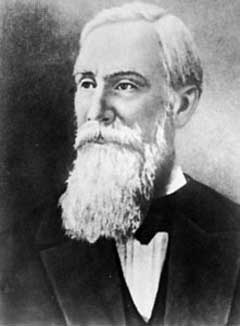
\includegraphics[width=0.7\textwidth]{Chebyshev}
\end{column}
\end{columns}
\begin{align*}
&a_n(\mathbf{x}) = (2 - \delta_{0n})J_n(\mathbf{x})\\
&T_n(\mathbf{X}) = 2\mathbf{X}T_{n-1}(\mathbf{X}) - T_{n-2}(\mathbf{X}) \qquad T_0(\mathbf{X}) = \mathbf{I} \quad T_1(\mathbf{X}) = \mathbf{X}
\end{align*}

\begin{itemize}
  \color{green}
  \item Very parallelizable (GEMM)
  \item O$(N^3)$ scaling (with better prefactor than diagonalization)
  \item Better round off than Taylor series at any given order
\end{itemize}
\begin{itemize}
  \color{red}
  \item ????
\end{itemize}

\end{frame}

\begin{frame}
\frametitle{Clever Trick for Matrix Series Expansions}
\blfootnote{DBWY; Goings, J.J; Li. X.; \emph{JCTC}. \textbf{2016}, 7, 4501.}

At any even order, $N$,  a matrix series expansion may be cut in half
\begin{equation*}
\sum_n^N c_n \mathbf{X}^n = \sum_n^{N/2} c_n \mathbf{X}^n + \mathbf{X}^{N/2}\sum_n^{N/2} c_{n+N/2}\mathbf{X}^n
\end{equation*}
~\\
~\\

{ \bf
Only requires explicit formation of matrix powers up to $N/2$!
}
\begin{itemize}
  \item Fewer GEMM operations ($N/2 + 1$ as opposed to $N$)
  \item Less opportunity for error propagation through repeated floating point operations.
\end{itemize}
\end{frame}


\begin{frame}
\frametitle{Clever Trick for Matrix Series Expansions}

\textbf{Taylor Series Expansion:}
\begin{equation*}
c_k = \frac{(-2\mathrm{i}\Delta t)^k}{k!}
\end{equation*}

\textbf{Chebyshev Expansion:}
\begin{equation*}
c_k = \text{ ??}
\end{equation*}
\begin{itemize}
  \item Each term in expansion depends on $T_k$ which non-trivially is related to $X^k$.
  \item \bf Current form requires full $N$ GEMM operations!
\end{itemize}
\end{frame}

\begin{frame}
\frametitle{Unrolling the Chebyshev Expansion}
\blfootnote{DBWY; Goings, J.J; Li. X.; \emph{JCTC}. \textbf{2016}, 7, 4501.}

Clearly, $T_n$ depends maximally on $X^n$, but also on all other $X^k$ $k < n$.

\begin{equation*}
\sum_n^N c_n(\tilde{\alpha}) \mathbf{\tilde{X}}^n = \sum_n^N  a_n(\tilde{\alpha})T_n(-\mathrm{i}\tilde{\mathbf{X}})
\end{equation*}

\begin{align*}
&T_2(x) = 2x^2 - 1\\
&T_3(x) = 4x^3 - 3x\\
&T_4(x) = 8x^4 - 8x^2 + 1
\end{align*}

\begin{equation*}
\sum = 8a_4x^4 + 4\mathrm{i}a_3x^3 - (2a_2 + 8a_4)x^2 + (3\mathrm{i}a_3 - \mathrm{i}a_1)x
\end{equation*}

\end{frame}


\begin{frame}
\frametitle{Unrolling the Chebyshev Expansion}
\blfootnote{http://oeis.org/}
\blfootnote{DBWY; Goings, J.J; Li. X.; \emph{JCTC}. \textbf{2016}, 7, 4501.}

It turns out (via OEIS...) that this is a geometric progression with a closed form expression,
thus,
\begin{equation*}
c_k(\mathbf{x}) = \sum_{n = k}^K a_n(\mathbf{x}) \zeta(n,k)
\end{equation*}
\begin{equation*}
\zeta(n,k) = \begin{cases}
0 & (k+n)\text{ odd or } n < k \\
1 & k = 0 \text{ and } n \text{ even}\\
\frac{2^{k-1}n}{k} \begin{pmatrix} \frac{n+k}{2} - 2 \\ k - 1\end{pmatrix} & \text{else}
\end{cases}
\end{equation*}

\end{frame}

\begin{frame}
\frametitle{Performance of the Nonrecursive Chebyshev Propagator}
\blfootnote{DBWY; Goings, J.J; Li. X.; \emph{JCTC}. \textbf{2016}, 7, 4501.}

\vspace{-1cm}
\begin{columns}
\begin{column}{0.5\textwidth}
\begin{figure}
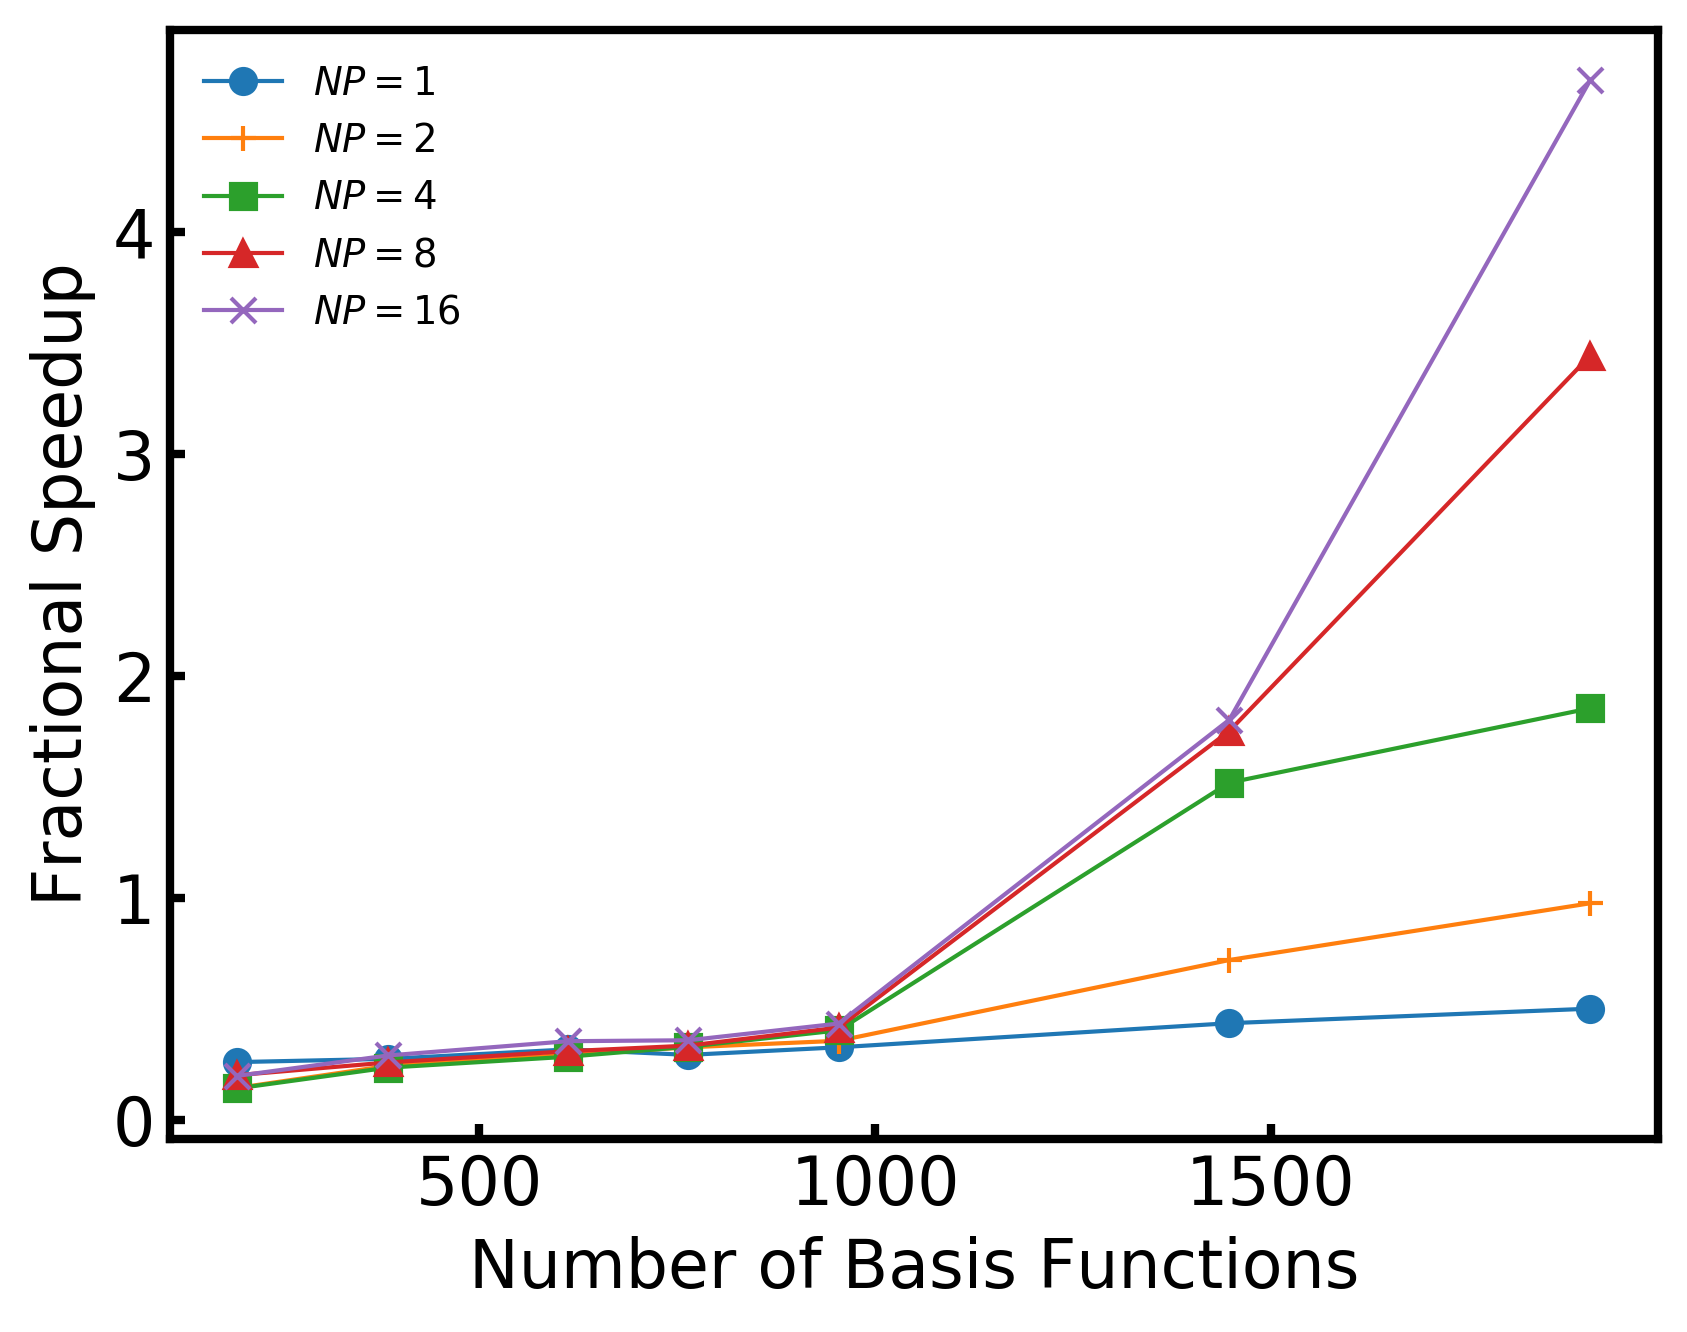
\includegraphics[width=\textwidth]{Speedup_1000.png}
\caption{\footnotesize Parallel performance of the Chebyshev propagator as a relative speedup over eigen decomposition.}
\end{figure}
\end{column}
\begin{column}{0.5\textwidth}
\begin{figure}
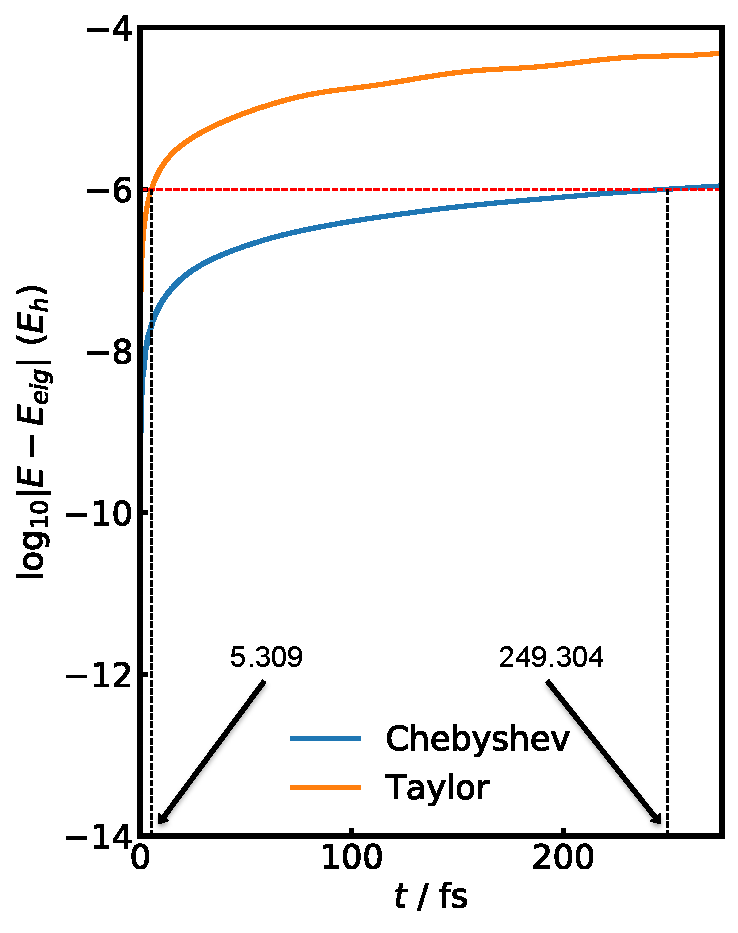
\includegraphics[width=0.8\textwidth]{Error2WAnnote}
\caption{\footnotesize Comparison of error accumulation between Taylor and Chebyshev expansions of the quantum propagator}
\end{figure}
\end{column}
\end{columns}
\vspace{-1cm}
\end{frame}





\end{document}
